\begin{figure}
\begin{subfigure}{0.475\textwidth}
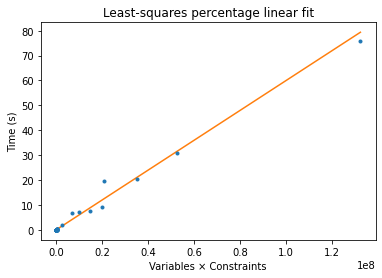
\includegraphics[width=0.9\textwidth]{images/least-squares.png}
\caption{\solve, \RecCheck execution time vs. $\norm{V}\norm{C}$ (blue dots), linear model (orange line)}
\label{fig:stats:linregress}
\end{subfigure}
\hfill
\begin{subfigure}{0.475\textwidth}
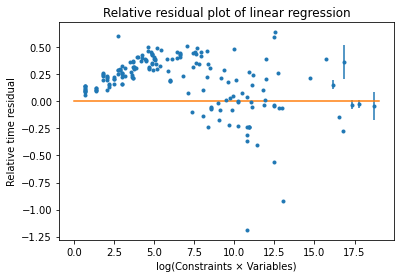
\includegraphics[width=0.9\textwidth]{images/relative-residuals.png}
\caption{Relative residuals plot (log scale)}
\label{fig:stats:residuals}
\end{subfigure}
\\ \hfill \\
\begin{subfigure}{0.475\textwidth}
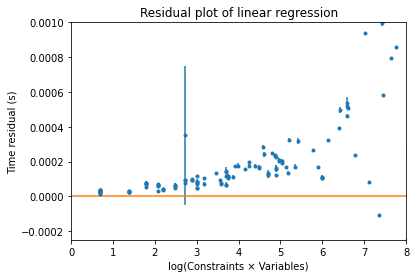
\includegraphics[width=0.9\textwidth]{images/residuals.png}
\caption{Residuals plot, $\log(\norm{V}\norm{C}) < 8$ (log scale)}
\label{fig:stats:residuals-zoom}
\end{subfigure}
\hfill
\begin{subfigure}{0.475\textwidth}
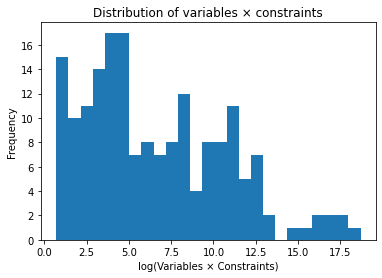
\includegraphics[width=0.9\textwidth]{images/distribution.png}
\caption{Distribution of $\norm{V}\norm{C}$, 25 bins (log scale)}
\label{fig:stats:vcs-distr}
\end{subfigure}
\caption{}
\label{fig:stats}
\end{figure}
